\begin{frame}
	\frametitle{Longo Prazo}
	\begin{itemize}
		\setlength\itemsep{1em}
		\item Ao longo prazo todos os factores produtivos se alteram e, assim, n\~ao existem custos fixos.
		\item A empresa tem mais alternativas e pode tomar decis\~oes que lhe estavam vedadas no curto prazo.
	\end{itemize}
\end{frame}

\begin{frame}
	\frametitle{Problema da empresa a longo prazo}
		Determinar a melhor combina\c c\~ao de $K$ e $L$ que permitem obter dada produ\c c\~ao ($Q^*$) ao menor custo: 
		\begin{align*}
			Min_{K,L}\ &rK+wL\\
			 s.a.\ &F(K,L)=Q^*
		\end{align*}
\end{frame}

\begin{frame}
	\frametitle{$F(K,L)=Q^*$}
	\begin{itemize}
		\setlength\itemsep{1em}
		\item A condi\c c\~ao $F(K,L)=Q^*$ representa todas as combina\c c\~oes de $K$ e $L$ que permitem atingir a mesma quantidade produzida. Definem uma \textbf{isoquanta}, isto \'e, uma curva de n\'ivel da fun\c c\~ao $F(K,L)$ ao n\'ivel de $Q^*$.
		\item Graficamente, para fun\c c\~oes de produ\c c\~ao da fam\'ilia $F(K,L)=AK^aL^b$ uma isoquanta \'e uma hip\'erbole no espa\c co ($K,L$).
	\end{itemize}
\end{frame}

\begin{frame}
	\frametitle{$F(K,L)=Q^*$}
	\begin{center}
		\begin{tikzpicture}[
			scale = 1,
			every node/.style = {scale = 1}
			]

			\draw[thick,->] (-0.1,0) -- (5.1,0)node[below]{$L$};
			\draw[thick,->] (0,-0.1) -- (0,5.1)node[left]{$K$};

			\draw (0.5,3.5) to [bend right] (3,0.5)node[right]{$Q^*$};
			\draw (1,4) to [bend right] (3.5,1)node[right]{$Q^{**}$};
			\draw (1.5,4.5) to [bend right] (4,1.5)node[right]{$Q^{***}$};

		\end{tikzpicture}
	\end{center}
\end{frame}

\begin{frame}
	\frametitle{Exemplo}
	Se a fun\c c\~ao de produ\c c\~ao for \[Q=K^{0.5}L^{0.5}\]

	No espa\c co $(L,K)$ todas as combina\c c\~oes de capital e trabalho que permitem atingir a produ\c c\~ao $Q=100$ podem ser representadas pela \emph{\textbf{isoquanta}} de equa\c c\~ao:\[100=K^{0.5}L^{0.5}\] ou seja $L=\frac{10,000}{K}$
\end{frame}

\begin{frame}
	\frametitle{Exemplo}
	Ent\~ao para obter a produ\c c\~ao $Q=100$ de forma a minimizar custos ($K$ e $L$) qual a melhor combina\c c\~ao de factores? Se admitirmos que cada factor \'e remunerado a 5um por unidade, o problema do produtor ser\'a 
	\begin{align*}
		\min_{K,L} \ 5K+5L\\
		s.a. \ 100=K^{0.5}L^{0.5}
	\end{align*}

	Proceder por substitui\c c\~ao, da restri\c c\~ao obtemos $K$, ou $L$, reemplazamos na fun\c c\~ao a optimizar, e resolvemos agora s\'o com uma vari\'avel!

\end{frame}

\begin{frame}
	\frametitle{Exemplo}
	Por substitui\c c\~ao de vari\'avel, \'e f\'acil obter: \(L=\frac{10,000}{K}\), e logo \[CT(K)=5K+5\times\frac{10,000}{K}\]
	O m\'inimo de $CT$ em $K$ obter-se-\'a com a derivada em zero (CPO):
	\begin{align*}
		\frac{\partial CT}{\partial K}=5-\frac{50,000}{K^2}=0 \ \Rightarrow \ K^2 = 10,000 \ \Rightarrow \ K = 100
	\end{align*}
	Logo $L=100$, e $CT=1,000$ no \'optimo.
\end{frame}

\begin{frame}
	\frametitle{Isocusto}

	\begin{tcolorbox}[title=\textbf{Isocusto},colback=iscal_color!20!white,colframe=iscal_color]
		Recta formada por todas as combina\c c\~oes de $K$ e $L$ que t\^em o mesmo custo total: \[\overline{CT}=r\times K + w\times L\]
	\end{tcolorbox}

	No exemplo, essa recta tem equa\c c\~ao $1,000=5K+5L$

	\vspace{0.5cm}

	Graficamente, tangencia a \textbf{Isoquanta} $L=\frac{10,000}{K}$ no ponto \'optimo $K=100$, $L=100$

\end{frame}

\begin{frame}
	\frametitle{\(100 = K^{0.5}L^{0.5}\) \\  \(1,000 = 5K+5L\)}
	\begin{center}
		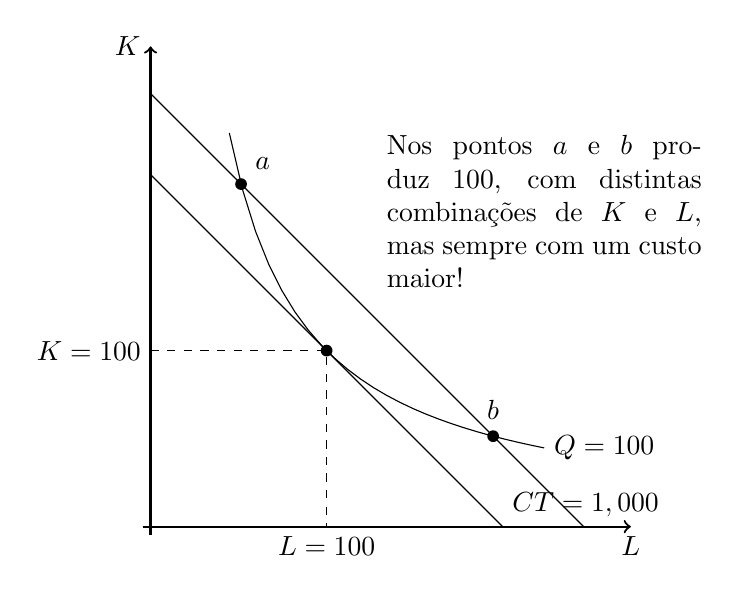
\begin{tikzpicture}[
			scale = 1,
			every node/.style = {scale = 1},
			declare function = {
				iq(\x) = 5/\x;
				ic(\a,\x) = \a-\x;
			}
			]

			\def\w{4.472}
			\def\ww{5.5}
			\def\eq{2.236}

			\draw[thick,->] (-0.1,0) -- (6.1,0)node[below]{$L$};
			\draw[thick,->] (0,-0.1) -- (0,6.1)node[left]{$K$};

			\onslide<2->{
				\draw [domain=1:5,variable=\x] plot (\x,{iq(\x)})node[right]{$Q=100$};
				\draw [domain=0:\w,variable=\x] plot (\x,{ic(\w,\x)});
			}

			\onslide<2-3>{
				\draw(\w,{ic(\w,\w)})node[above right]{$CT=1,000$};
			}

			\onslide<3->{
				\draw[dashed](0,{iq(\eq)})node[left]{$K=100$} -- (\eq,{iq(\eq)}) node[circle,fill,inner sep=1.5 pt]{} -- (\eq,0)node[below]{$L=100$};
			}

			\def\la{1.1492}
			\def\lb{4.3508}

			\onslide<4->{
				\draw [domain=0:\ww,variable=\x] plot (\x,{ic(\ww,\x)});
				\draw (\la,{ic(\ww,\la)})node[circle,fill,inner sep=1.5pt,label=above right:{$a$}]{};
				\draw (\lb,{ic(\ww,\lb)})node[circle,fill,inner sep=1.5pt,label=above:{$b$}]{};
				\draw (5,4)node{\parbox{4cm}{Nos pontos $a$ e $b$ produz 100, com distintas combina\c c\~oes de $K$ e $L$, mas sempre com um custo maior!}};
			}



		\end{tikzpicture}
	\end{center}
\end{frame}

\begin{frame}
	\frametitle{Os custos de longo prazo s\~ao menores}
	\begin{center}
		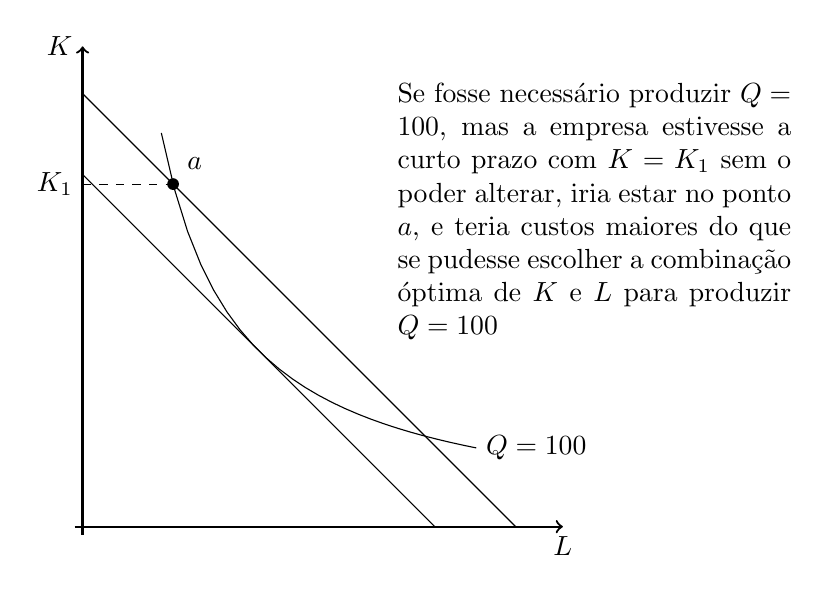
\begin{tikzpicture}[
			scale = 1,
			every node/.style = {scale = 1},
			declare function = {
				iq(\x) = 5/\x;
				ic(\a,\x) = \a-\x;
			}
			]

			\def\w{4.472}
			\def\ww{5.5}
			\def\eq{2.236}

			\draw[thick,->] (-0.1,0) -- (6.1,0)node[below]{$L$};
			\draw[thick,->] (0,-0.1) -- (0,6.1)node[left]{$K$};

			\draw [domain=1:5,variable=\x] plot (\x,{iq(\x)})node[right]{$Q=100$};
			\draw [domain=0:\w,variable=\x] plot (\x,{ic(\w,\x)});
			%\draw(\w,{ic(\w,\w)})node[above right]{$CT=1,000$};
			%\draw[dashed](0,{iq(\eq)})node[left]{$K=100$} -- (\eq,{iq(\eq)}) node[circle,fill,inner sep=1.5 pt]{} -- (\eq,0)node[below]{$L=100$};

			\def\la{1.1492}
			\def\lb{4.3508}

			\draw [domain=0:\ww,variable=\x] plot (\x,{ic(\ww,\x)});
			\draw (\la,{ic(\ww,\la)})node[circle,fill,inner sep=1.5pt,label=above right:{$a$}]{};
			%\draw (\lb,{ic(\ww,\lb)})node[circle,fill,inner sep=1.5pt,label=above:{$b$}]{};
			\draw (6.5,4)node{\parbox{5cm}{Se fosse necess\'ario produzir $Q=100$, mas a empresa estivesse a curto prazo com $K=K_1$ sem o poder alterar, iria estar no ponto $a$, e teria custos maiores do que se pudesse escolher a combina\c c\~ao \'optima de $K$ e $L$ para produzir $Q=100$}};

			\draw[dashed](0,{ic(\ww,\la)})node[left]{$K_1$} -- (\la,{ic(\ww,\la)});

		\end{tikzpicture}
	\end{center}
\end{frame}


\begin{frame}
	\frametitle{Custos de longo prazo}
	\begin{itemize}
		\setlength\itemsep{1em}
		\item A longo prazo, a empresa escolhe as quantidades economicamente eficientes de trabalho e capital que minimizam o custo da produ\c c\~ao de uma dada quantidade a colocar no mercado, que por sua vez depende das exig\^encias do mercado impostas pela procura e pela concorr\^encia que a empresa enfrenta
		\item \textbf{...ent\~ao, a longo prazo os custos m\'edios ser\~ao sempre menores ou iguais aos custos de curto prazo}
	\end{itemize}
\end{frame}

\begin{frame}
	\frametitle{Custos m\'edios a longo prazo}
	\begin{center}
		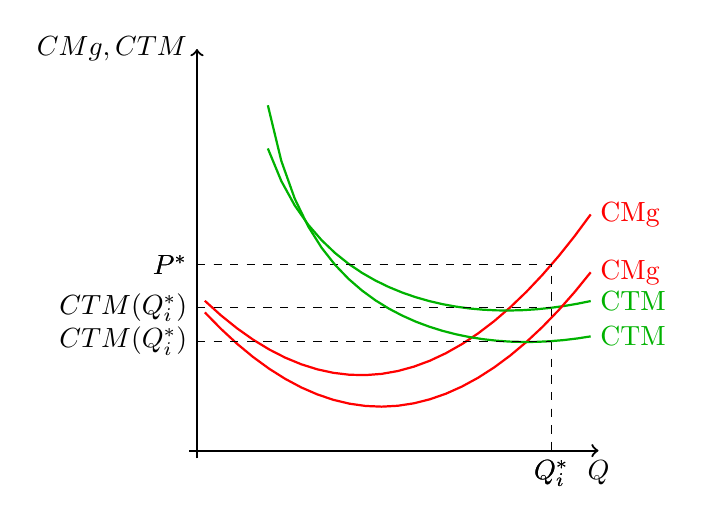
\begin{tikzpicture}[
			scale = 1,
			every node/.style = {scale = 1},
			declare function = {
				cv(\x) = \x - (1/4)*\x^2 + (1/25)*\x^3;
				cf(\x) = 1;
				ct(\x) = cv(\x) + cf(\x);
				cmg(\x) = 1 - (2/4)*\x + (3/25)*\x^2;
				ctm(\x) = ct(\x)/\x;
				cmg2(\x) = 0.8 - (2/4)*(\x-0.25) + (3/25)*(\x-0.25)^2;
				ctm2(\x) = ct(\x-0.25)/(\x-0.25)-0.2;
				cvm(\x) = cv(\x)/\x;
			}]

			\def\p{4.5}

			\draw[->,thick] (-0.1,-0) -- (5.1,-0) node[below]{$Q$};
			\draw[->,thick] (0,-0.1) -- (0,5.1) node[left]{$CMg,CTM$};

			\onslide<1>{

				\draw[red,thick,domain=0.1:5,variable=\x] plot (\x,{2*cmg(\x)-0});
				\draw[red](5,{2*cmg(5)-0})node[right]{CMg};

				\draw[dashed] (0,{2*cmg(\p)})node[left]{$P^*$} -- (\p,{2*cmg(\p)}) -- (\p,0)node[below]{$Q_i^*$};		

				\draw[green!70!black,thick,domain=0.9:5,variable=\x] plot (\x,{2*ctm(\x)-0});
				\draw[green!70!black](5,{2*ctm(5)-0})node[right]{CTM};

				\draw[dashed] (0,{2*ctm(\p)})node[left]{$CTM(Q_i^*)$} -- (\p,{2*ctm(\p)});

			}

			\onslide<2>{

				\draw[opacity=0.2,red,domain=0.1:5,variable=\x] plot (\x,{2*cmg(\x)-0});
				\draw[opacity=0.2,red](5,{2*cmg(5)-0})node[right]{CMg};

				\draw[dashed] (0,{2*cmg(\p)})node[left]{$P^*$} -- (\p,{2*cmg(\p)}) -- (\p,0)node[below]{$Q_i^*$};		

				\draw[opacity=0.2,green!70!black,domain=0.9:5,variable=\x] plot (\x,{2*ctm(\x)-0});
				\draw[opacity=0.2,green!70!black](5,{2*ctm(5)-0})node[right]{CTM};

				\draw[opacity=0.2,dashed] (0,{2*ctm(\p)})node[left]{$CTM(Q_i^*)$} -- (\p,{2*ctm(\p)});

				%==========================================================================

				\draw[red,thick,domain=0.1:5,variable=\x] plot (\x,{2*cmg2(\x)-0});
				\draw[red](5,{2*cmg2(5)-0})node[right]{CMg};		

				\draw[green!70!black,thick,domain=0.9:5,variable=\x] plot (\x,{2*ctm2(\x)-0});
				\draw[green!70!black](5,{2*ctm2(5)-0})node[right]{CTM};

				\draw[dashed] (0,{2*ctm2(\p)})node[left]{$CTM(Q_i^*)$} -- (\p,{2*ctm2(\p)});

			}

		\end{tikzpicture}
	\end{center}
\end{frame}

\begin{frame}
	\frametitle{Custos m\'edios a longo prazo}
	\begin{center}
		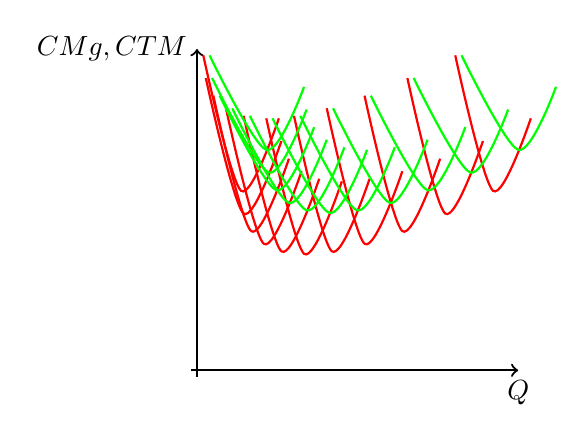
\begin{tikzpicture}[
			scale = 0.8,
			every node/.style = {scale = 1}
			]

			\draw[->,thick] (-0.1,-0) -- (5.1,-0) node[below]{$Q$};
			\draw[->,thick] (0,-0.1) -- (0,5.1) node[left]{$CMg,CTM$};

			\def\con{50}
			\def\conx{50}
			\def\powx{2}
			\def\pow{2}

			\foreach \r in {-50,-40,...,50}{
				\draw[thick,red] plot [smooth] coordinates {
					({0.1+((\r+50)/\conx)^\powx},{4+(\r/\con)^\pow})
					({0.7+((\r+50)/\conx)^\powx},{1.85+(\r/\con)^\pow})
					({1.3+((\r+50)/\conx)^\powx},{3+(\r/\con)^\pow})
					};
			
			}

			\foreach \r in {-50,-40,...,50}{
				\draw[thick,green] plot [smooth] coordinates {
					({0.2+((\r+50)/\conx)^\powx},{4+(\r/\con)^\pow})
					({1.1+((\r+50)/\conx)^\powx},{2.5+(\r/\con)^\pow})
					({1.7+((\r+50)/\conx)^\powx},{3.5+(\r/\con)^\pow})
					};
			}

		\end{tikzpicture}
	\end{center}
\end{frame}

\begin{frame}
	\frametitle{Custos m\'edios a longo prazo}
	\begin{center}
		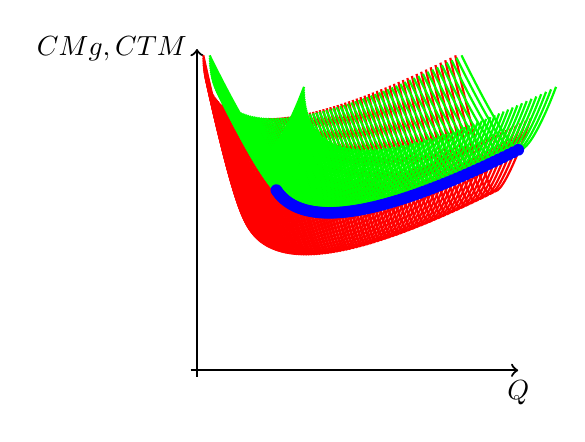
\begin{tikzpicture}[
			scale = 0.8,
			every node/.style = {scale = 1}
			]

			\draw[->,thick] (-0.1,-0) -- (5.1,-0) node[below]{$Q$};
			\draw[->,thick] (0,-0.1) -- (0,5.1) node[left]{$CMg,CTM$};

			\def\con{50}
			\def\conx{50}
			\def\powx{2}
			\def\pow{2}

			\onslide<1-2>{
				\foreach \r in {-50,...,50}{
					\draw[thick,red] plot [smooth] coordinates {
						({0.1+((\r+50)/\conx)^\powx},{4+(\r/\con)^\pow})
						({0.7+((\r+50)/\conx)^\powx},{1.85+(\r/\con)^\pow})
						({1.3+((\r+50)/\conx)^\powx},{3+(\r/\con)^\pow})
						};
				
				}

				\foreach \r in {-50,...,50}{
					\draw[thick,green] plot [smooth] coordinates {
						({0.2+((\r+50)/\conx)^\powx},{4+(\r/\con)^\pow})
						({1.1+((\r+50)/\conx)^\powx},{2.5+(\r/\con)^\pow})
						({1.7+((\r+50)/\conx)^\powx},{3.5+(\r/\con)^\pow})
						};
				}
			}

			\onslide<2-3>{
				\foreach \r in {-30,...,50}{
					\draw({1.1+((\r+50)/\conx)^\powx},{2.5+(\r/\con)^\pow}) node[circle,blue,fill,inner sep=1.5pt]{};
				}
			}

		\end{tikzpicture}
	\end{center}
	\onslide<3>{Curva de Custo M\'edio de Longo Prazo}
\end{frame}

\begin{frame}
	\frametitle{Observa\c c\~ao}
	\begin{itemize}
		\item Os custos aqui referidos s\~ao \textbf{custos econ\'omicos}, ou seja s\~ao \textbf{custos de oportunidade} , que j\'a sabemos inclu\'irem outros valores para al\'em da despesa de quisi\c c\~ao dos fatores de produ\c c\~ao
		\item ent\~ao: um lucro econ\'omico ser\'a sempre n\~ao superior ao lucro contabil\'istico, presente nas Demonstra\c c\~oes de Resultados! Porqu\^e?
		\item Recordar o conceito de Custo de Oportunidade!
	\end{itemize}
\end{frame}

\begin{frame}
	\frametitle{Economias de Escala}
	\begin{itemize}
		\item Enquanto $CM_{LP}$ for decrescente, diz-se que h\'a Economias de Escala
		\item Quando $CM_{LP}$ \'e crescente, diz-se que h\'a Deseconomias de Escala
		\item O m\'inimo de $CM_{LP}$ \'e a Escala M\'inima Eficiente. O n\'ivel de $Q$ onde esse m\'inimo ocorre \'e espec\'ifico \`a tecnologia/sector de atividade.
	\end{itemize}
\end{frame}

\begin{frame}
	\frametitle{Economias de Escala}
	\begin{center}
		\begin{tikzpicture}[
			scale = 1,
			every node/.style = {scale = 0.8}
			]

			\draw[->,thick] (-0.1,-0) -- (5.1,-0) node[below]{$Q$};
			\draw[->,thick] (0,-0.1) -- (0,5.1) node[left]{$CM$};

			\draw[thick,red,domain=0.5:5,variable=\x] plot (\x,{((\x-2.5)/1.5)^2+0.5})node[right]{$CM_{LP}$};
			\draw[dashed] (2.5,0)node[below]{$Q^*$} -- (2.5,4);

			\draw[pen colour={blue},ultra thick,decorate,decoration={calligraphic brace,mirror},yshift=-0.5cm] (0,0) -- (2.5,0) node[midway,yshift=-0.75cm]{\parbox{2cm}{Economias de Escala}};
			\draw[pen colour={blue},ultra thick,decorate,decoration={calligraphic brace,mirror},yshift=-0.5cm] (2.5,0) -- (5,0) node[midway,yshift=-0.75cm]{\parbox{2cm}{Deseconomias de Escala}};

		\end{tikzpicture}

		Escala M\'inima Eficiente \\ (corresponde a um determinado valor de $K$)
	\end{center}
\end{frame}

\begin{frame}
	\frametitle{Economias de Escala}
	O n\'ivel de $Q$ que minimiza $CM_{LP}$ influencia o n\'umero de empresas (e respectiva dimens\~ao ao n\'ivel de volume de \emph{output}) em cada sector/mercado.

	\vspace{0.5cm}

	Quanto menor a quantidade que minimiza o $CM_{LP}$ maior \'e a tend\^encia para haver mais empresas de menor dimens\~ao, para satisfazer um mercado com uma dada procura

\end{frame}

\begin{frame}
	\frametitle{Concorr\^encia Perfeita (Longo Prazo)}
	Se $\Pi>0$, o mercado \'e atraente: entram mais empresas, expandindo a oferta:
	\begin{center}
		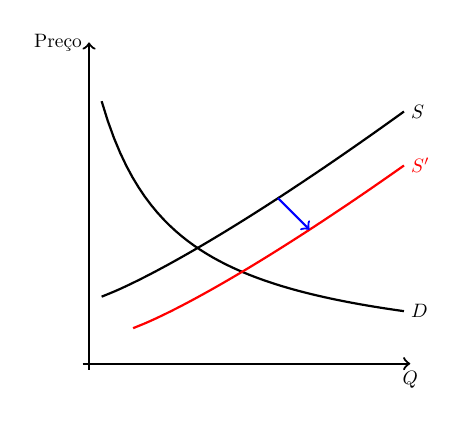
\begin{tikzpicture}[
			scale = 0.8,
			every node/.style = {scale = 0.7},
			declare function = {
				s(\x) = 1+(\x/2)^(3/2.5);
				s2(\x) = s(\x-0.5)-0.5;
				d(\x) = 5/(\x+1);
				d2(\x) = d(\x-0.5)+0.5;
			}
			]

			\def\ea{0.75}
			\def\eb{2.80397}
			\def\eq{1.72301}
			\def\noeq{3.04638}
			\def\neweq{2.42959}

			\draw[thick,->] (-0.1,0) -- (5.1,0)node[below]{$Q$};
			\draw[thick,->] (0,-0.1) -- (0,5.1)node[left]{Pre\c co};

			\draw[thick,samples=50,domain=0.2:5,variable=\x] plot (\x,{d(\x)})node[right]{$D$};
			\draw[thick,samples=50,domain=0.2:5,variable=\x] plot (\x,{s(\x)})node[right]{$S$};
			\draw[red,thick,samples=50,domain=0.7:5,variable=\x] plot (\x,{s2(\x)})node[right]{$S'$};

			\draw[->,blue,thick] (3,{s(3)}) -- (3.5,{s2(3.5)});

		\end{tikzpicture}
	\end{center}
	Baixa o pre\c co de equil\'ibrio, aumenta a quantidade, mas cada empresa produz um pouco menos do que antes, porque h\'a mais empresas no mercado... diminui o lucro individual!
\end{frame}

\begin{frame}
	\frametitle{Entrada de Empresas no Mercado}

	\begin{center}
		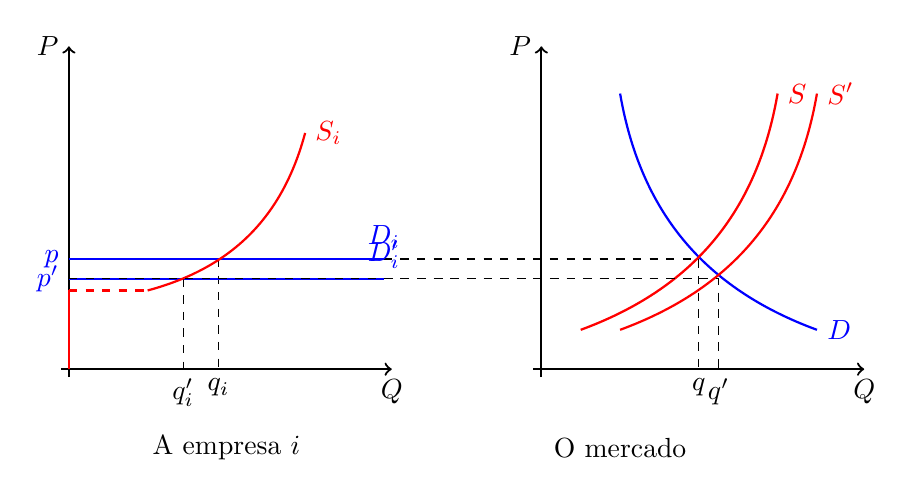
\begin{tikzpicture}[
			scale = 1,
			every node/.style = {scale = 1}
			]

			\def\p{1.4}
			\def\pa{1.15}
			\def\q{8}
			\def\qi{1.9}
			\def\qia{1.45}
			\def\qa{8.25}
			

			\draw[thick,->] (-0.1,0) -- (4.1,0) node[below]{$Q$};
			\draw[thick,->] (5.9,0) -- (10.1,0) node[below]{$Q$};

			\draw[thick,->] (0,-0.1) -- (0,4.1) node[left]{$P$};
			\draw[thick,->] (6,-0.1) -- (6,4.1) node[left]{$P$};

			\onslide<1-3>{
				\draw[thick,blue] (0,\p)node[left]{$p$} -- (4,\p)node[above]{$D_i$};
				\draw[dashed] (\qi,\p) -- (\qi,0)node[below]{$q_i$};
				\draw[dashed] (4,\p) -- (\q,\p) -- (\q,0)node[below]{$q$};
			}

			\onslide<4->{
				\draw[opacity=0.2,thick,blue] (0,\p)node[left]{$p$} -- (4,\p)node[above]{$D_i$};
				\draw[opacity=0.2,dashed] (\qi,\p) -- (\qi,0)node[below]{$q_i$};
				\draw[opacity=0.2,dashed] (4,\p) -- (\q,\p) -- (\q,0)node[below]{$q$};

				\draw[thick,blue] (0,\pa)node[left]{$p'$} -- (4,\pa)node[above]{$D_i'$};
				\draw[dashed] (\qia,\pa) -- (\qia,0)node[below]{$q_i'$};
				\draw[dashed] (4,\pa) -- (\qa,\pa) -- (\qa,0)node[below]{$q'$};
			}

			\draw[red,thick] (1,1) to [bend right] (3,3) node[right]{$S_i$};
			\draw[red,thick] (0,0) -- (0,1);
			\draw[dashed,thick,red] (0,1) -- (1,1);

			\draw[blue,thick] (7,3.5) to [bend right] (9.5,0.5)node[right]{$D$};
			
			\onslide<1-3>{
				\draw[red,thick] (6.5,0.5) to [bend right] (9,3.5)node[right]{$S$};
			}

			\onslide<3->{
				\draw[opacity=0.2,red,thick] (6.5,0.5) to [bend right] (9,3.5)node[right]{$S$};
			}

			\draw(2,-1) node {A empresa $i$};
			\draw(7,-1) node {O mercado};

			\onslide<2->{
				\draw[red,thick] (7,0.5) to [bend right] (9.5,3.5)node[right]{$S'$};				
			}

			\onslide<3->{
				\draw[dashed](0,\pa) -- (\qa,\pa)--(\qa,0);
			}

		\end{tikzpicture}
	\end{center}
	Entram empresas $\rightarrow$ h\'a expans\~ao da oferta $\rightarrow$ pre\c co desce $\rightarrow$ quantidade produzida por cada empresa desce $\rightarrow$ no total, h\'a mais produto no mercado $\rightarrow$ o lucro individual diminui
	
\end{frame}

\begin{frame}
	\frametitle{Equil\'ibrio de Longo Prazo}
	Entrar\~ao empresas no mercado (sair\~ao, caso $\Pi<0$) at\'e que se verifique $\Pi=0$, pelo que o equil\'ibrio de $LP$ \'e tal que: \[p=Cmg_{LP}=CM_{LP}\]
\end{frame}

\begin{frame}
	\frametitle{Equil\'ibrio de Longo Prazo}
	\begin{center}
		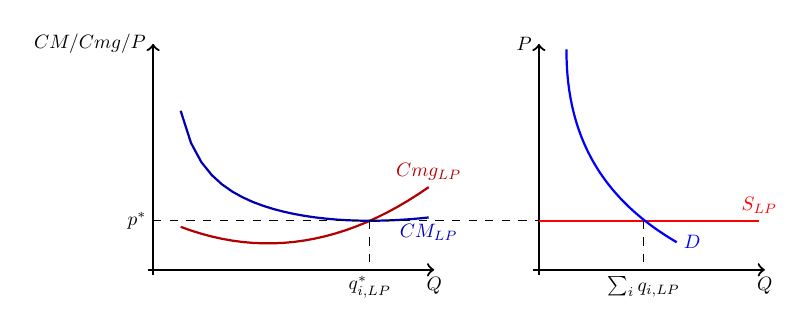
\begin{tikzpicture}[
			scale = 0.7,
			every node/.style = {scale = 0.7},
			declare function = {
				cv(\x) = \x - (1/4)*\x^2 + (1/25)*\x^3;
				cf(\x) = 1;
				ct(\x) = cv(\x) + cf(\x);
				cmg(\x) = 1 - (2/4)*\x + (3/25)*\x^2;
				ctm(\x) = ct(\x)/\x;
				cvm(\x) = cv(\x)/\x;
			}]			

			\def\qs{3.9331}
			\def\qt{8.9}

			\draw[thick,->] (-0.1,0) -- (5.1,0) node[below]{$Q$};
			\draw[thick,->] (6.9,0) -- (11.1,0) node[below]{$Q$};

			\draw[thick,->] (0,-0.1) -- (0,4.1) node[left]{$CM/Cmg/P$};
			\draw[thick,->] (7,-0.1) -- (7,4.1) node[left]{$P$};

			\draw [thick,red!70!black,domain=0.5:5, variable=\x] plot(\x,{cmg(\x)})node[above]{$Cmg_{LP}$};
			\draw [thick,blue!70!black,domain=0.5:5, variable=\x] plot(\x,{ctm(\x)})node[below]{$CM_{LP}$};

			\draw[dashed] (0,{cmg(\qs)})node[left]{$p^*$} -- (7,{cmg(\qs)});
			\draw[dashed] (\qs,{cmg(\qs)}) -- (\qs,0)node[below]{$q^*_{i,LP}$};
			\draw[red,thick] (7,{cmg(\qs)}) -- (11,{cmg(\qs)})node[above]{$S_{LP}$};

			\draw[blue,thick](7.5,4) to [bend right] (9.5,0.5)node[right]{$D$};
			\draw[dashed] (\qt,{cmg(\qs)})--(\qt,0)node[below]{$\sum_{i}q_{i,LP}$};

		\end{tikzpicture}
	\end{center}
	LP: todo o escedente econ\'omico do mercado \'e o Excedente do Consumidor!
\end{frame}